

\section{Coordinated Cross-device Inference}
\label{sec:design-sys}
This section describes \sys-sys, the \sys-PIM integrated AFD system with hardware-software co-design to achieve high throughput, 
addressing the challenges of inter-device data and progress synchronization overheads.


\begin{figure}[t]
  \setlength{\abovecaptionskip}{2pt}
  \setlength{\belowcaptionskip}{-10pt}
  \centering
    \begin{minipage}[t]{\linewidth}
    \centering
    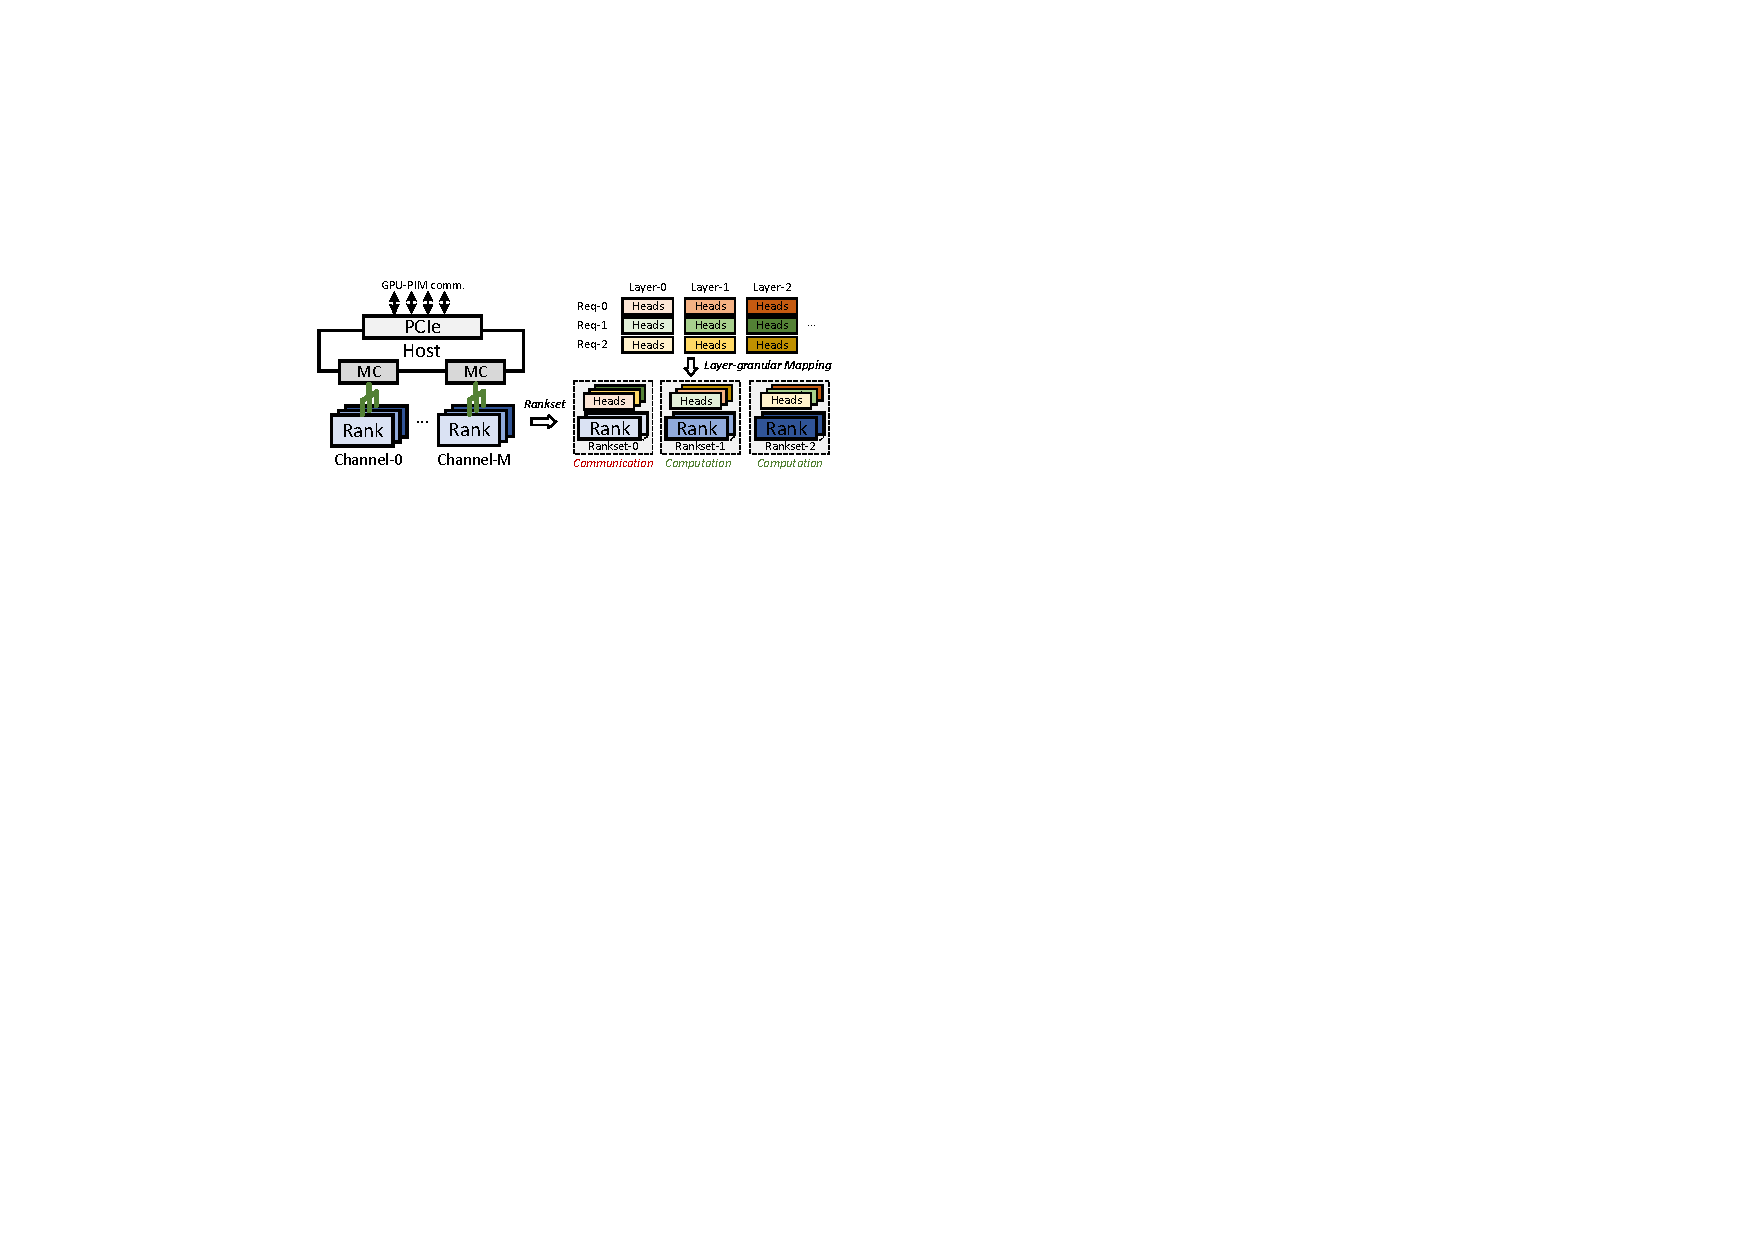
\includegraphics[width=\textwidth]{figs/design-rankset.pdf}
    \footnotesize
    \end{minipage}
    \caption{\textbf{Hiding data transfer overhead with rankset-granular communication computation overlapping.}}
  \label{fig:design-zigzag-rankset}
\end{figure}

\begin{figure*}[t]
  \setlength{\abovecaptionskip}{-1pt}
  \setlength{\belowcaptionskip}{-5pt}
  \centering
    \begin{minipage}[t]{0.9\linewidth}
    \centering
    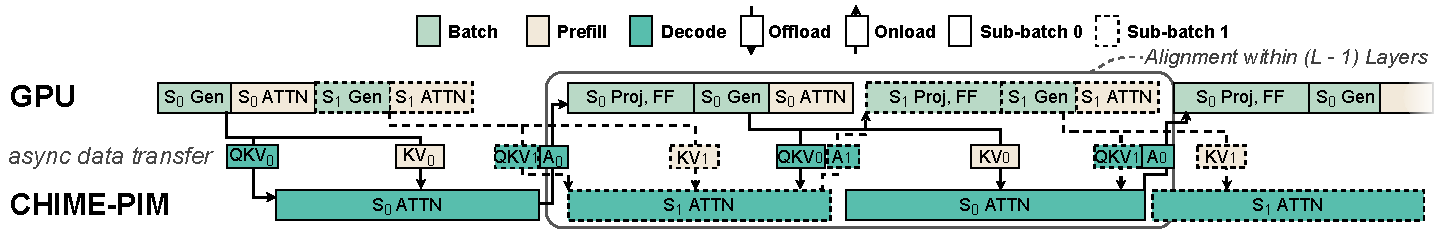
\includegraphics[width=\textwidth]{figs/design-zigzag.pdf}
    \footnotesize
    \end{minipage}
    \caption{\textbf{Coordinating cross-device inference with \sys-sys.} 
        \textit{\sys hides the communication cost and aligns the parallel executions across devices. ``ATTN'' denotes decoding or prefilling attention, ``Gen'' denotes QKV Generation and ``Proj, FF'' denotes the projection and feed-forward operations.}
        }
  \label{fig:design-compute-graph}
\end{figure*}





\subsection{Rankset-granular Comm-Comp Overlapping}
\label{sec:design-sys-comm}
Data synchronization between the GPU and \sys-PIM includes transferring the following data:
(1) prefilling KVs (proportional to the lengths of inputs); 
(2) decoding QKV (a token for each request), and (3) decoding attention results (a token for each request). 
Ideally, with sub-batch scheduling, the data can be transferred asynchronously, e.g., sending the decoding QKV for a sub-batch when executing the other sub-batch.
However, GPU-PIM data communication and attention computation on the \sys-PIM share the memory buses, which indicates that the communication would block the computation.
This blocking prevents asynchronous data transfer, incurring non-negligible overhead since the PCIe bandwidth~\cite{pci2025pci} could be orders of magnitude lower than that of \sys-PIM (Table~\ref{tab:simulator}).

We identify that the challenge arises from the coarse granularity, i.e., treating all ranks as a whole, for doing either communication or computation.
The key to address the challenge is finding the finest granularity of independent and concurrent communication and computation.




\myparagraph{Rankset-granular communication-computation overlapping.}
Our key observation is that, \emph{due to the shared memory buses, only one rank can be accessed in a channel at the same time during communication, while other ranks remain idle.}
This motivates our proposal of the \emph{rankset}, 
which is composed of one rank from every channel, forming the basic granularity of independent communication and computation.
In this case, a rankset is the minimum set of ranks to fully utilize all channels.
As shown in Fig.~\ref{fig:design-zigzag-rankset}, each channel has three ranks, forming three ranksets.
During the communication of one rankset, other ranksets can perform independent computation without blocking, 
which could preserve 2/3 of computational power during communication.


Moreover, we achieve \emph{rankset-granular load balance} leveraging the feature of \emph{identical KV cache sizes among layers}. 
Specifically, we store the KV cache of each request at the granularity of layers in an interleaved manner.
It ensures load balance of each rankset transfers, avoiding the rankset transferring the most data slows down the overall progress.













\subsection{Alignment Predicting Scheduling}
\label{sec:sys-scheduler}
To prevent idle bubbles caused by synchronizing the progress of parallel operations across the two devices, 
the key for \sys's scheduler is to properly select requests to form sub-batches, \emph{aligning the execution latencies of parallel operations on the two devices}.
However, LLM's auto-regressive nature makes the alignment challenging, since the execution latencies could vary with factors such as the number of processed tokens, the batch sizes, etc. 
Prior AFD systems fall short in achieving that goal:
for HBM-PIM-based AFD systems~\cite{park2024attacc,heo2024neupims}, the latencies on the PIM side could always be smaller than that on the GPU (as shown in Fig.~\ref{fig:intro-motiv}-b).
For CPU-based AFD systems~\cite{jiang2024neo}, they lack modeling the execution latencies of each operation when scheduling.
Moreover, the computation time on the CPU side can be interfered by other CPU applications and may lack predictability~\cite{christina2013paragon,liu2024jiagu,lo2015heracles}. 

\myparagraph{Opportunity of performance modeling.}
To address the challenge, \sys proposes \emph{Alignment-predicting scheduling}, 
whose key feature is modeling and predicting the execution latencies on the two devices that helps to align the parallel execution latencies. 
Leveraging the feature, it selects requests to form sub-batches, whose predicted latencies on the two devices are aligned, as shown in Fig.~\ref{fig:design-compute-graph}.
\sys exploits the following opportunities to achieve performance predictability.
First, the execution with the \sys-PIM is \emph{interference-free.}  
Second, the factors that affect the batch performances (e.g., the batch size, number of processed tokens, etc.) are known in advance.
Third, abundant prior works have explored methods for predicting the execution on the GPU~\cite{cui2021abacus,gujarati2020clockwork,yang2022infless}.


\subsection{Implementation Details for Scheduling}
\myparagraph{Model features.}
\sys describes a sub-batch $i$ with following arguments: 
$c_{p_{i}}$, the list of chunk sizes of each prefilling request;
$f_{p_{i}}$, the list of finished token numbers of each prefilling request;
$f_{d_{i}}$, the list of finished token numbers (on each rank) of each decoding request.
The latencies of both sub-batches can be modeled as follows: %
\begin{align}
  \label{equ:obj_1} &T_{{\rm GPU}_{0}} = t_{p}(c_{p_{0}}, f_{p_{0}}) + t_{\rm batch}(c_{p_{0}}, f_{d_{1}}) \\
  \label{equ:obj_2} &T_{{\rm PIM}_{0}} = t_{d}(f_{d_{0}}) + t_{\rm comm}(f_{d_{0}}, c_{p_{1}}) \\
  \label{equ:obj_3} &T_{{\rm GPU}_{1}} = t_{p}(c_{p_{1}}, f_{p_{1}}) + t_{\rm batch}(c_{p_{1}}, f_{d_{0}}) \\
  \label{equ:obj_4} &T_{{\rm PIM}_{1}} = t_{d}(f_{d_{1}}) + t_{\rm comm}(f_{d_{1}}, c_{p_{0}})
\end{align}
Equation~\ref{equ:obj_1},\ref{equ:obj_3} denotes the latency on the GPU side, which contains the latency of prefilling attention and batched FC operations.
Equation~\ref{equ:obj_2},\ref{equ:obj_4} denotes the latency on the \sys-PIM in the granularity of rank, which contains the latency of decoding attention, and overlapped data transfer overheads.

\myparagraph{Scheduling policy.}
With the following steps, the scheduling policy selects requests to form sub-batches with aligned parallel cross-device execution:
\begin{enumerate}
  \item Add one prefilling request into each sub-batch. When there is no prefilling request, skip the step.
  \item For each prefilling request added (which implies an increase in $T_{GPU}$), \sys adds $N$ decoding requests to each sub-batch and assign them to ranks in a load balancing manner. After that, it predicts $T_{PIM}$ and $T_{GPU}$ for each sub-batch. If $T_{PIM} < T_{GPU}$, it adds another $N$ decoding requests until $T_{PIM} > T_{GPU}$. 
  \item If there are remaining prefill requests, it repeats step (1) until the PIM memory is exhausted. 
  When the memory is saturated and the bubble is on the PIM side, the last prefilling request of each sub-batch is chunked, dynamically adjusting $T_{\rm GPU}$ to make it as close as possible to the $T_{\rm PIM}$ of the other sub-batch. 
\end{enumerate}

The larger the value of $N$, 
the coarser the granularity of batch execution time adjustment, 
but the more beneficial it is for achieving load balance among ranks for requests. 
In our implementation, since MHA has more heads and these heads can be evenly distributed across chips, the $N$ for MHA is set to 1, while the $N$ for GQA is set to 16.

\myparagraph{Model selection.}
\label{sec:runtime-profiling}
Now we describe how \sys models the execution latencies of various inference operations.
First, to model $T_{\rm GPU}$, we leverage Random Forest Regression (RFR) for its three advantages: capability of incremental learning, low latency, and high accuracy.
The efficiency of RFR for execution latency prediction has been proven in many prior works~\cite{liu2024jiagu,zhao2021gsight}, and it is open to use other models that feature similarly.
Second, to model $T_{\rm PIM}$, given that \sys-PIM execution is featured predictable (i.e., execution time is linearly related to the number of computed/transferred tokens),
we can use a simple and fast linear model for $t_{\rm comm}$ and each rank's $t_{d}$.
The overall $t_{d}$ is determined by the rank with the longest execution time.
The models can be described with the following formula (take sub-batch 0 as an example):
\begin{align*}
  &T_{{\rm PIM}_{0}} = {\rm Linear}(\sum{f_{d_{0}}}, {\rm len}(f_{d_{0}}), \sum{c_{p_{1}}}) \\
  &T_{{\rm GPU}_{0}} = {\rm RFR}_{p}(c_{p_{0}}, f_{p_{0}}) + {\rm RFR}_{\rm batch}(\sum{c_{p_{0}}}, {\rm len}(f_{d_{0}}))
\end{align*}

\myparagraph{Runtime profiling.}
\sys applies runtime profiling, which collects the latency information and corresponding batch information during inference.
The dataset maintained by \sys dynamically evolves with the collected data for incrementally updating the model, thereby adapting to changing execution environment.
Moreover, we evaluate the prediction models of the \sys scheduler by splitting the collected 1000 data points into training and test sets in an 8:2 ratio. 
The experimental results show that our model exhibits great performance predictability, achieving prediction relative errors of less than $\sim$1\% (median value $<$ 0.5\%).

















